\documentclass[twoside]{book}

% Packages required by doxygen
\usepackage{fixltx2e}
\usepackage{calc}
\usepackage{doxygen}
\usepackage[export]{adjustbox} % also loads graphicx
\usepackage{graphicx}
\usepackage[utf8]{inputenc}
\usepackage{makeidx}
\usepackage{multicol}
\usepackage{multirow}
\PassOptionsToPackage{warn}{textcomp}
\usepackage{textcomp}
\usepackage[nointegrals]{wasysym}
\usepackage[table]{xcolor}

% NLS support packages
\usepackage[T2A]{fontenc}
\usepackage[magyar]{babel}

% Font selection
\usepackage[T1]{fontenc}
\usepackage[scaled=.90]{helvet}
\usepackage{courier}
\usepackage{amssymb}
\usepackage{sectsty}
\renewcommand{\familydefault}{\sfdefault}
\allsectionsfont{%
  \fontseries{bc}\selectfont%
  \color{darkgray}%
}
\renewcommand{\DoxyLabelFont}{%
  \fontseries{bc}\selectfont%
  \color{darkgray}%
}
\newcommand{\+}{\discretionary{\mbox{\scriptsize$\hookleftarrow$}}{}{}}

% Page & text layout
\usepackage{geometry}
\geometry{%
  a4paper,%
  top=2.5cm,%
  bottom=2.5cm,%
  left=2.5cm,%
  right=2.5cm%
}
\tolerance=750
\hfuzz=15pt
\hbadness=750
\setlength{\emergencystretch}{15pt}
\setlength{\parindent}{0cm}
\setlength{\parskip}{3ex plus 2ex minus 2ex}
\makeatletter
\renewcommand{\paragraph}{%
  \@startsection{paragraph}{4}{0ex}{-1.0ex}{1.0ex}{%
    \normalfont\normalsize\bfseries\SS@parafont%
  }%
}
\renewcommand{\subparagraph}{%
  \@startsection{subparagraph}{5}{0ex}{-1.0ex}{1.0ex}{%
    \normalfont\normalsize\bfseries\SS@subparafont%
  }%
}
\makeatother

% Headers & footers
\usepackage{fancyhdr}
\pagestyle{fancyplain}
\fancyhead[LE]{\fancyplain{}{\bfseries\thepage}}
\fancyhead[CE]{\fancyplain{}{}}
\fancyhead[RE]{\fancyplain{}{\bfseries\leftmark}}
\fancyhead[LO]{\fancyplain{}{\bfseries\rightmark}}
\fancyhead[CO]{\fancyplain{}{}}
\fancyhead[RO]{\fancyplain{}{\bfseries\thepage}}
\fancyfoot[LE]{\fancyplain{}{}}
\fancyfoot[CE]{\fancyplain{}{}}
\fancyfoot[RE]{\fancyplain{}{\bfseries\scriptsize Készítette Doxygen }}
\fancyfoot[LO]{\fancyplain{}{\bfseries\scriptsize Készítette Doxygen }}
\fancyfoot[CO]{\fancyplain{}{}}
\fancyfoot[RO]{\fancyplain{}{}}
\renewcommand{\footrulewidth}{0.4pt}
\renewcommand{\chaptermark}[1]{%
  \markboth{#1}{}%
}
\renewcommand{\sectionmark}[1]{%
  \markright{\thesection\ #1}%
}

% Indices & bibliography
\usepackage{natbib}
\usepackage[titles]{tocloft}
\setcounter{tocdepth}{3}
\setcounter{secnumdepth}{5}
\makeindex

% Hyperlinks (required, but should be loaded last)
\usepackage{ifpdf}
\ifpdf
  \usepackage[pdftex,pagebackref=true]{hyperref}
\else
  \usepackage[ps2pdf,pagebackref=true]{hyperref}
\fi
\hypersetup{%
  colorlinks=true,%
  linkcolor=blue,%
  citecolor=blue,%
  unicode%
}

% Custom commands
\newcommand{\clearemptydoublepage}{%
  \newpage{\pagestyle{empty}\cleardoublepage}%
}

\usepackage{caption}
\captionsetup{labelsep=space,justification=centering,font={bf},singlelinecheck=off,skip=4pt,position=top}

%===== C O N T E N T S =====

\begin{document}

% Titlepage & ToC
\hypersetup{pageanchor=false,
             bookmarksnumbered=true,
             pdfencoding=unicode
            }
\pagenumbering{alph}
\begin{titlepage}
\vspace*{7cm}
\begin{center}%
{\Large My Project }\\
\vspace*{1cm}
{\large Készítette Doxygen 1.8.13}\\
\end{center}
\end{titlepage}
\clearemptydoublepage
\pagenumbering{roman}
\tableofcontents
\clearemptydoublepage
\pagenumbering{arabic}
\hypersetup{pageanchor=true}

%--- Begin generated contents ---
\chapter{Hierarchikus mutató}
\section{Osztályhierarchia}
Majdnem (de nem teljesen) betűrendbe szedett leszármazási lista\+:\begin{DoxyCompactList}
\item \contentsline{section}{Five\+In\+A\+Row.\+Five\+In\+A\+Row\+Test}{\pageref{class_five_in_a_row_1_1_five_in_a_row_test}}{}
\item Action\+Listener\begin{DoxyCompactList}
\item \contentsline{section}{Five\+In\+A\+Row.\+Board}{\pageref{class_five_in_a_row_1_1_board}}{}
\end{DoxyCompactList}
\item J\+Panel\begin{DoxyCompactList}
\item \contentsline{section}{Five\+In\+A\+Row.\+Game}{\pageref{class_five_in_a_row_1_1_game}}{}
\begin{DoxyCompactList}
\item \contentsline{section}{Five\+In\+A\+Row.\+Board}{\pageref{class_five_in_a_row_1_1_board}}{}
\item \contentsline{section}{Five\+In\+A\+Row.\+Five\+In\+A\+Row}{\pageref{class_five_in_a_row_1_1_five_in_a_row}}{}
\end{DoxyCompactList}
\end{DoxyCompactList}
\item Mouse\+Listener\begin{DoxyCompactList}
\item \contentsline{section}{Five\+In\+A\+Row.\+Board}{\pageref{class_five_in_a_row_1_1_board}}{}
\end{DoxyCompactList}
\end{DoxyCompactList}

\chapter{Osztálymutató}
\section{Osztálylista}
Az összes osztály, struktúra, unió és interfész listája rövid leírásokkal\+:\begin{DoxyCompactList}
\item\contentsline{section}{\hyperlink{class_five_in_a_row_1_1_board}{Five\+In\+A\+Row.\+Board} }{\pageref{class_five_in_a_row_1_1_board}}{}
\item\contentsline{section}{\hyperlink{class_five_in_a_row_1_1_five_in_a_row}{Five\+In\+A\+Row.\+Five\+In\+A\+Row} }{\pageref{class_five_in_a_row_1_1_five_in_a_row}}{}
\item\contentsline{section}{\hyperlink{class_five_in_a_row_1_1_five_in_a_row_test}{Five\+In\+A\+Row.\+Five\+In\+A\+Row\+Test} }{\pageref{class_five_in_a_row_1_1_five_in_a_row_test}}{}
\item\contentsline{section}{\hyperlink{class_five_in_a_row_1_1_game}{Five\+In\+A\+Row.\+Game} }{\pageref{class_five_in_a_row_1_1_game}}{}
\end{DoxyCompactList}

\chapter{Osztályok dokumentációja}
\hypertarget{class_five_in_a_row_1_1_board}{}\section{Five\+In\+A\+Row.\+Board osztályreferencia}
\label{class_five_in_a_row_1_1_board}\index{Five\+In\+A\+Row.\+Board@{Five\+In\+A\+Row.\+Board}}
A Five\+In\+A\+Row.\+Board osztály származási diagramja\+:\begin{figure}[H]
\begin{center}
\leavevmode
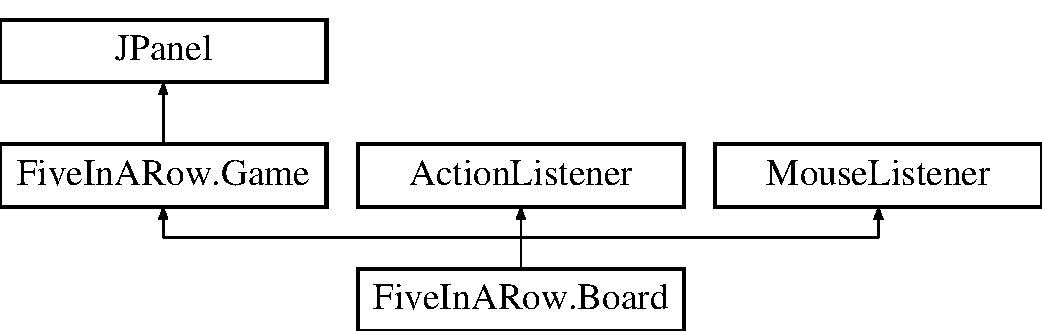
\includegraphics[height=3.000000cm]{class_five_in_a_row_1_1_board}
\end{center}
\end{figure}
\subsection*{Publikus tagfüggvények}
\begin{DoxyCompactItemize}
\item 
\hyperlink{class_five_in_a_row_1_1_board_a2b70fd89cd3cdc2debe8765e02c822b7}{Board} ()  throws I\+O\+Exception
\item 
void \hyperlink{class_five_in_a_row_1_1_board_ac350a7dcbd91c4cf0874d0e2009c4312}{action\+Performed} (Action\+Event evt)
\item 
void \hyperlink{class_five_in_a_row_1_1_board_a1c804beb7b1edce3b6f218cf38aa7ee8}{do\+Click\+Square} (int row, int col)  throws I\+O\+Exception 
\item 
boolean \hyperlink{class_five_in_a_row_1_1_board_aea2974ecd2423b50869c18fac52939ca}{winner} (int row, int col)
\item 
void \hyperlink{class_five_in_a_row_1_1_board_a1cf86000d5a69acc39c4033a978bd80e}{paint\+Component} (Graphics g)
\item 
void \hyperlink{class_five_in_a_row_1_1_board_a4e208e8945037bcc95d0d6682276c071}{draw\+Win\+Line} (Graphics g)
\item 
void \hyperlink{class_five_in_a_row_1_1_board_aa153513650cd323723cde3bf652de3c6}{mouse\+Pressed} (Mouse\+Event evt)
\item 
\mbox{\Hypertarget{class_five_in_a_row_1_1_board_ab6a8f59222e0a160a8214f249291553a}\label{class_five_in_a_row_1_1_board_ab6a8f59222e0a160a8214f249291553a}} 
void {\bfseries mouse\+Released} (Mouse\+Event evt)
\item 
\mbox{\Hypertarget{class_five_in_a_row_1_1_board_a449742085f2fee47d54286942dbe27bd}\label{class_five_in_a_row_1_1_board_a449742085f2fee47d54286942dbe27bd}} 
void {\bfseries mouse\+Clicked} (Mouse\+Event evt)
\item 
\mbox{\Hypertarget{class_five_in_a_row_1_1_board_ae5469b6c4ee446f2a91ace532773715d}\label{class_five_in_a_row_1_1_board_ae5469b6c4ee446f2a91ace532773715d}} 
void {\bfseries mouse\+Entered} (Mouse\+Event evt)
\item 
\mbox{\Hypertarget{class_five_in_a_row_1_1_board_a99158ac51edd0b007fe77841ee4b5dcc}\label{class_five_in_a_row_1_1_board_a99158ac51edd0b007fe77841ee4b5dcc}} 
void {\bfseries mouse\+Exited} (Mouse\+Event evt)
\end{DoxyCompactItemize}
\subsection*{Additional Inherited Members}


\subsection{Részletes leírás}
Megjelen�ti a t�bl�t ami 168$\ast$168 pixel m�ret� n�gyzetr�csos t�bla, 2pixel m�ret� v�laszt�kkal. Azt felt�telezve, hogy az ablak 172$\ast$172 pixel m�ret�. Ez az oszt�ly v�gzi a f� munk�t amikor a j�t�kosok j�tszanak �s megjelen�ti a t�bl�t. Ebben a programban a t�bla amin a j�t�k zajlik 13 sorb�l �s 13 oszlopb�l �ll� n�gyzetr�cs.

\begin{DoxyAuthor}{Szerző}
Roland 
\end{DoxyAuthor}


\subsection{Konstruktorok és destruktorok dokumentációja}
\mbox{\Hypertarget{class_five_in_a_row_1_1_board_a2b70fd89cd3cdc2debe8765e02c822b7}\label{class_five_in_a_row_1_1_board_a2b70fd89cd3cdc2debe8765e02c822b7}} 
\index{Five\+In\+A\+Row\+::\+Board@{Five\+In\+A\+Row\+::\+Board}!Board@{Board}}
\index{Board@{Board}!Five\+In\+A\+Row\+::\+Board@{Five\+In\+A\+Row\+::\+Board}}
\subsubsection{\texorpdfstring{Board()}{Board()}}
{\footnotesize\ttfamily Five\+In\+A\+Row.\+Board.\+Board (\begin{DoxyParamCaption}{ }\end{DoxyParamCaption}) throws I\+O\+Exception}

Konstruktor. L�trehozza a gombokat �s a c�mk�t. Figyeli az eg�r kattint�st �s a gombokra kattint�st. Elind�tja a j�t�kot. 
\begin{DoxyExceptions}{Kivételek}
{\em I\+O\+Exception} & Hiba eset�n I\+O\+Exceptiont dob. \\
\hline
\end{DoxyExceptions}


\subsection{Tagfüggvények dokumentációja}
\mbox{\Hypertarget{class_five_in_a_row_1_1_board_ac350a7dcbd91c4cf0874d0e2009c4312}\label{class_five_in_a_row_1_1_board_ac350a7dcbd91c4cf0874d0e2009c4312}} 
\index{Five\+In\+A\+Row\+::\+Board@{Five\+In\+A\+Row\+::\+Board}!action\+Performed@{action\+Performed}}
\index{action\+Performed@{action\+Performed}!Five\+In\+A\+Row\+::\+Board@{Five\+In\+A\+Row\+::\+Board}}
\subsubsection{\texorpdfstring{action\+Performed()}{actionPerformed()}}
{\footnotesize\ttfamily void Five\+In\+A\+Row.\+Board.\+action\+Performed (\begin{DoxyParamCaption}\item[{Action\+Event}]{evt }\end{DoxyParamCaption})}

Reag�l a felhaszn�l� kattint��s�ra a 3 gomb szerint. \mbox{\Hypertarget{class_five_in_a_row_1_1_board_a1c804beb7b1edce3b6f218cf38aa7ee8}\label{class_five_in_a_row_1_1_board_a1c804beb7b1edce3b6f218cf38aa7ee8}} 
\index{Five\+In\+A\+Row\+::\+Board@{Five\+In\+A\+Row\+::\+Board}!do\+Click\+Square@{do\+Click\+Square}}
\index{do\+Click\+Square@{do\+Click\+Square}!Five\+In\+A\+Row\+::\+Board@{Five\+In\+A\+Row\+::\+Board}}
\subsubsection{\texorpdfstring{do\+Click\+Square()}{doClickSquare()}}
{\footnotesize\ttfamily void Five\+In\+A\+Row.\+Board.\+do\+Click\+Square (\begin{DoxyParamCaption}\item[{int}]{row,  }\item[{int}]{col }\end{DoxyParamCaption}) throws I\+O\+Exception}

Ez a met�dus eg�r kattint�sra h�v�dik. A \hyperlink{class_five_in_a_row_1_1_board_aa153513650cd323723cde3bf652de3c6}{mouse\+Pressed()} met�dus �ltal, amikor a j�t�kos a t�bl�n l�v� n�gyzetekre kattint. A met�dus h�v�sa csak akkor t�rt�nik meg ha a j�t�k folyamatban van. A row param�ter a sorokat. A col param�ter az oszlopokat jel�li. 
\begin{DoxyParams}{Paraméterek}
{\em row} & A row a t�bla sorait jel�li. \\
\hline
{\em col} & A col a t�bla oszlopait jel�li. \\
\hline
\end{DoxyParams}

\begin{DoxyExceptions}{Kivételek}
{\em I\+O\+Exception} & Hiba esetln I\+O\+Exceptiont dob. \\
\hline
\end{DoxyExceptions}
\mbox{\Hypertarget{class_five_in_a_row_1_1_board_a4e208e8945037bcc95d0d6682276c071}\label{class_five_in_a_row_1_1_board_a4e208e8945037bcc95d0d6682276c071}} 
\index{Five\+In\+A\+Row\+::\+Board@{Five\+In\+A\+Row\+::\+Board}!draw\+Win\+Line@{draw\+Win\+Line}}
\index{draw\+Win\+Line@{draw\+Win\+Line}!Five\+In\+A\+Row\+::\+Board@{Five\+In\+A\+Row\+::\+Board}}
\subsubsection{\texorpdfstring{draw\+Win\+Line()}{drawWinLine()}}
{\footnotesize\ttfamily void Five\+In\+A\+Row.\+Board.\+draw\+Win\+Line (\begin{DoxyParamCaption}\item[{Graphics}]{g }\end{DoxyParamCaption})}

2 pixel sz�les piros vonalat rajzol a n�gyzeteket keresztbe �th�zva a (win\+\_\+r1,win\+\_\+c1)t�l a (win\+\_\+r2, win\+\_\+c2)ig. Ez akkor h�vod meg amikor valamelyik j�t�kos megnyerte a j�t�kot. Teh�t kirakta az 5 azonos b�b�t egym�s mell�. A v�ltoz�k �rt�kei a count() met�dusban ker�lnek be�ll�t�sra. 
\begin{DoxyParams}{Paraméterek}
{\em g} & A g a Graphics oszt�ly objektuma. \\
\hline
\end{DoxyParams}
\mbox{\Hypertarget{class_five_in_a_row_1_1_board_aa153513650cd323723cde3bf652de3c6}\label{class_five_in_a_row_1_1_board_aa153513650cd323723cde3bf652de3c6}} 
\index{Five\+In\+A\+Row\+::\+Board@{Five\+In\+A\+Row\+::\+Board}!mouse\+Pressed@{mouse\+Pressed}}
\index{mouse\+Pressed@{mouse\+Pressed}!Five\+In\+A\+Row\+::\+Board@{Five\+In\+A\+Row\+::\+Board}}
\subsubsection{\texorpdfstring{mouse\+Pressed()}{mousePressed()}}
{\footnotesize\ttfamily void Five\+In\+A\+Row.\+Board.\+mouse\+Pressed (\begin{DoxyParamCaption}\item[{Mouse\+Event}]{evt }\end{DoxyParamCaption})}

Reag�l az felhaszn�l� �ltali eg�rkattint�sra. Ha nincs j�t�k folyamatban akkor error �zenetet mutat. Egy�bk�nt megadja, hogy a felhaszn�l� melyik sorba �s oszlopba kattintott �s megh�vja a \hyperlink{class_five_in_a_row_1_1_board_a1c804beb7b1edce3b6f218cf38aa7ee8}{do\+Click\+Square()} met�dust, ami kezeli ezt. \mbox{\Hypertarget{class_five_in_a_row_1_1_board_a1cf86000d5a69acc39c4033a978bd80e}\label{class_five_in_a_row_1_1_board_a1cf86000d5a69acc39c4033a978bd80e}} 
\index{Five\+In\+A\+Row\+::\+Board@{Five\+In\+A\+Row\+::\+Board}!paint\+Component@{paint\+Component}}
\index{paint\+Component@{paint\+Component}!Five\+In\+A\+Row\+::\+Board@{Five\+In\+A\+Row\+::\+Board}}
\subsubsection{\texorpdfstring{paint\+Component()}{paintComponent()}}
{\footnotesize\ttfamily void Five\+In\+A\+Row.\+Board.\+paint\+Component (\begin{DoxyParamCaption}\item[{Graphics}]{g }\end{DoxyParamCaption})}

Kirajzolja a t�bl�t �s a b�bukat a t�bl�n. Ha a j�t�kot valaki megynerte, akkor az 5 b�b�t tartalmaz� n�gyzetet �th�zza egy piros vonallal. \mbox{\Hypertarget{class_five_in_a_row_1_1_board_aea2974ecd2423b50869c18fac52939ca}\label{class_five_in_a_row_1_1_board_aea2974ecd2423b50869c18fac52939ca}} 
\index{Five\+In\+A\+Row\+::\+Board@{Five\+In\+A\+Row\+::\+Board}!winner@{winner}}
\index{winner@{winner}!Five\+In\+A\+Row\+::\+Board@{Five\+In\+A\+Row\+::\+Board}}
\subsubsection{\texorpdfstring{winner()}{winner()}}
{\footnotesize\ttfamily boolean Five\+In\+A\+Row.\+Board.\+winner (\begin{DoxyParamCaption}\item[{int}]{row,  }\item[{int}]{col }\end{DoxyParamCaption})}

Ez a met�dus mindig megh�v�dik amikor egy �j b�but raktak le a t�bl�ra. Ez hat�rozza meg, hogy az a l�p�s egy nyer� l�p�s volt-\/e vagy sem. Teh�t 5 azonos b�b� van-\/e egym�s mellett vagy sem. Mind a 4 lehets�ges ir�nyb�l megn�zi, hogy van e 5 ugyanolyan b�b� egym�s mellett a n�gyzetekben. Ha van 5 olyan n�gyzet ahol azonos b�b� van (vagy t�bb) akkor a j�t�k v�get �r �s a jelenlegi j�t�kos nyer. A row param�ter a sorokat, a col param�ter pedig az oszlopokat jel�li. 
\begin{DoxyParams}{Paraméterek}
{\em row} & A row a t�bla sorait jel�li. \\
\hline
{\em col} & A col a t�bla oszlopait jel�li. \\
\hline
\end{DoxyParams}
\begin{DoxyReturn}{Visszatérési érték}
Igazzal t�r vissza ha 5 ugyanolyan b�b�t tal�l egym�s mellett, k�l�nben hamissal. 
\end{DoxyReturn}


Ez a dokumentáció az osztályról a következő fájl alapján készült\+:\begin{DoxyCompactItemize}
\item 
Board.\+java\end{DoxyCompactItemize}

\hypertarget{class_five_in_a_row_1_1_five_in_a_row}{}\section{Five\+In\+A\+Row.\+Five\+In\+A\+Row osztályreferencia}
\label{class_five_in_a_row_1_1_five_in_a_row}\index{Five\+In\+A\+Row.\+Five\+In\+A\+Row@{Five\+In\+A\+Row.\+Five\+In\+A\+Row}}
A Five\+In\+A\+Row.\+Five\+In\+A\+Row osztály származási diagramja\+:\begin{figure}[H]
\begin{center}
\leavevmode
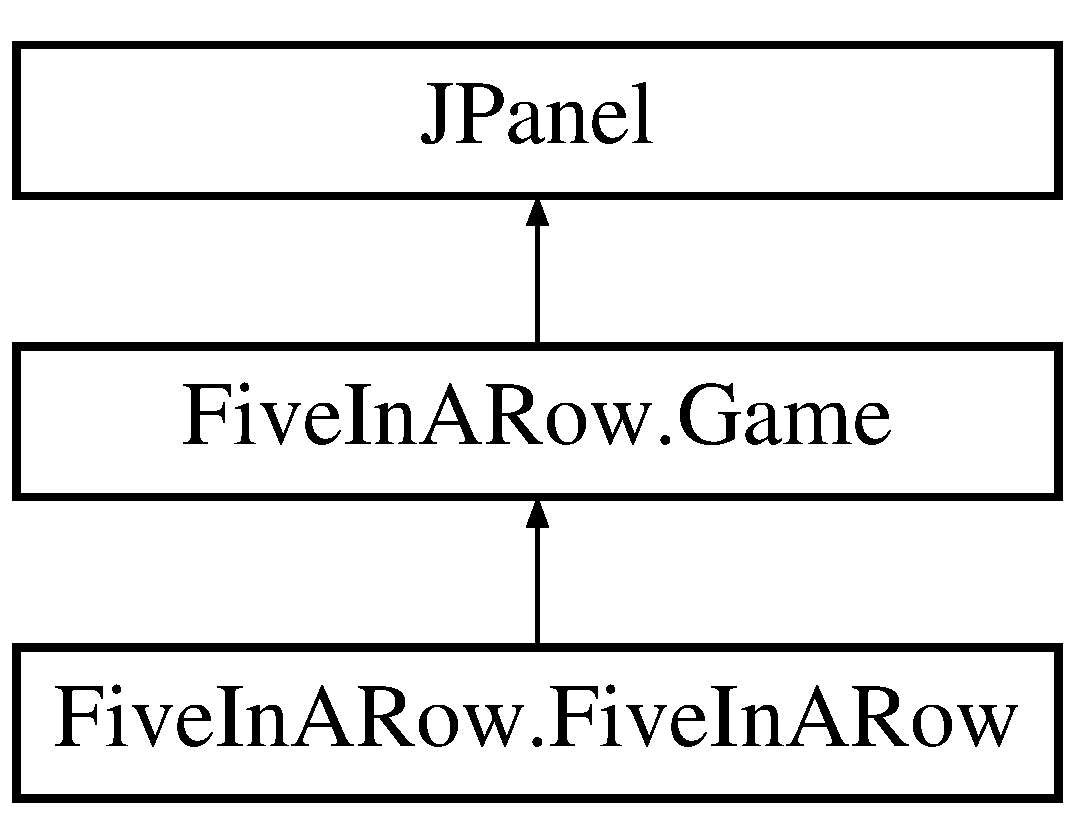
\includegraphics[height=3.000000cm]{class_five_in_a_row_1_1_five_in_a_row}
\end{center}
\end{figure}
\subsection*{Publikus tagfüggvények}
\begin{DoxyCompactItemize}
\item 
\hyperlink{class_five_in_a_row_1_1_five_in_a_row_a19a8181a1a9ca24c361258b39d426dea}{Five\+In\+A\+Row} ()  throws I\+O\+Exception
\end{DoxyCompactItemize}
\subsection*{Statikus publikus tagfüggvények}
\begin{DoxyCompactItemize}
\item 
static void \hyperlink{class_five_in_a_row_1_1_five_in_a_row_a0e1adc18a9e82c828626b03212de34da}{main} (String\mbox{[}$\,$\mbox{]} args)  throws I\+O\+Exception 
\end{DoxyCompactItemize}
\subsection*{Additional Inherited Members}


\subsection{Részletes leírás}
Ezzel a programmal k�t j�t�kos j�tszhat am�ba j�t�kot egym�s ellen. Mindig a fekete j�t�kos fogja kezdeni a j�t�kot. Amikor egy j�t�kos ki rak 5 b�but egym�s mell� a saj�tjai k�z�l, akkor nyer. A j�t�k d�ntetlennel �r v�get ha a t�bla megtelik azel�tt, hogy valamelyik j�t�kos nyer.

Az oszt�lynak van egy \hyperlink{class_five_in_a_row_1_1_five_in_a_row_a0e1adc18a9e82c828626b03212de34da}{main()} f�ggv�nye, amely seg�ts�g�vel tud a program �n�ll�an futni. A program megnyit egy ablakot (window) ami a \hyperlink{class_five_in_a_row_1_1_five_in_a_row}{Five\+In\+A\+Row} objektumot (object) haszn�lja.

\begin{DoxyAuthor}{Szerző}
Roland 
\end{DoxyAuthor}


\subsection{Konstruktorok és destruktorok dokumentációja}
\mbox{\Hypertarget{class_five_in_a_row_1_1_five_in_a_row_a19a8181a1a9ca24c361258b39d426dea}\label{class_five_in_a_row_1_1_five_in_a_row_a19a8181a1a9ca24c361258b39d426dea}} 
\index{Five\+In\+A\+Row\+::\+Five\+In\+A\+Row@{Five\+In\+A\+Row\+::\+Five\+In\+A\+Row}!Five\+In\+A\+Row@{Five\+In\+A\+Row}}
\index{Five\+In\+A\+Row@{Five\+In\+A\+Row}!Five\+In\+A\+Row\+::\+Five\+In\+A\+Row@{Five\+In\+A\+Row\+::\+Five\+In\+A\+Row}}
\subsubsection{\texorpdfstring{Five\+In\+A\+Row()}{FiveInARow()}}
{\footnotesize\ttfamily Five\+In\+A\+Row.\+Five\+In\+A\+Row.\+Five\+In\+A\+Row (\begin{DoxyParamCaption}{ }\end{DoxyParamCaption}) throws I\+O\+Exception}

A konstruktorban ker�l megtervez�sre a panel. A j�t�k f�r�sze a \hyperlink{class_five_in_a_row_1_1_game}{Game} �s a \hyperlink{class_five_in_a_row_1_1_board}{Board} oszt�lyban fut le. A m�retek �s a poz�ci�k be�ll�t�sa t�rt�nik itt �s a layout null-\/ra �ll�t�sa. 
\begin{DoxyExceptions}{Kivételek}
{\em I\+O\+Exception} & Hiba eset�n I\+O\+Exceptiont dob. \\
\hline
\end{DoxyExceptions}


\subsection{Tagfüggvények dokumentációja}
\mbox{\Hypertarget{class_five_in_a_row_1_1_five_in_a_row_a0e1adc18a9e82c828626b03212de34da}\label{class_five_in_a_row_1_1_five_in_a_row_a0e1adc18a9e82c828626b03212de34da}} 
\index{Five\+In\+A\+Row\+::\+Five\+In\+A\+Row@{Five\+In\+A\+Row\+::\+Five\+In\+A\+Row}!main@{main}}
\index{main@{main}!Five\+In\+A\+Row\+::\+Five\+In\+A\+Row@{Five\+In\+A\+Row\+::\+Five\+In\+A\+Row}}
\subsubsection{\texorpdfstring{main()}{main()}}
{\footnotesize\ttfamily static void Five\+In\+A\+Row.\+Five\+In\+A\+Row.\+main (\begin{DoxyParamCaption}\item[{String \mbox{[}$\,$\mbox{]}}]{args }\end{DoxyParamCaption}) throws I\+O\+Exception\hspace{0.3cm}{\ttfamily [static]}}

A main f�ggv�ny teszi lehet�v�, hogy a program �n�ll�an tudjon futni. Megnyit egy ablakot amin l�that� az am�ba t�bla, a program bez�r�dik amikor a felhaszn�l� bez�rja azt.


\begin{DoxyParams}{Paraméterek}
{\em args} & sztringek t�mbje \\
\hline
\end{DoxyParams}

\begin{DoxyExceptions}{Kivételek}
{\em I\+O\+Exception} & hiba eseten I\+O\+Exceptiont dob. \\
\hline
\end{DoxyExceptions}


Ez a dokumentáció az osztályról a következő fájl alapján készült\+:\begin{DoxyCompactItemize}
\item 
Five\+In\+A\+Row.\+java\end{DoxyCompactItemize}

\hypertarget{class_five_in_a_row_1_1_five_in_a_row_test}{}\section{Five\+In\+A\+Row.\+Five\+In\+A\+Row\+Test osztályreferencia}
\label{class_five_in_a_row_1_1_five_in_a_row_test}\index{Five\+In\+A\+Row.\+Five\+In\+A\+Row\+Test@{Five\+In\+A\+Row.\+Five\+In\+A\+Row\+Test}}
\subsection*{Publikus tagfüggvények}
\begin{DoxyCompactItemize}
\item 
\mbox{\Hypertarget{class_five_in_a_row_1_1_five_in_a_row_test_adf128eba6d432222a14f9d301ab55ab1}\label{class_five_in_a_row_1_1_five_in_a_row_test_adf128eba6d432222a14f9d301ab55ab1}} 
void {\bfseries set\+Up} ()
\item 
\mbox{\Hypertarget{class_five_in_a_row_1_1_five_in_a_row_test_a49bf96385805bd46340df2213c63f4d3}\label{class_five_in_a_row_1_1_five_in_a_row_test_a49bf96385805bd46340df2213c63f4d3}} 
void {\bfseries testwinner} ()
\item 
\mbox{\Hypertarget{class_five_in_a_row_1_1_five_in_a_row_test_acfd2d0ea7e0f3345eafaf55c3d565b4d}\label{class_five_in_a_row_1_1_five_in_a_row_test_acfd2d0ea7e0f3345eafaf55c3d565b4d}} 
void {\bfseries test\+Resign} ()
\item 
\mbox{\Hypertarget{class_five_in_a_row_1_1_five_in_a_row_test_ae760b4f8aed4884c9f7c60d3028538b3}\label{class_five_in_a_row_1_1_five_in_a_row_test_ae760b4f8aed4884c9f7c60d3028538b3}} 
void {\bfseries test\+Replay} ()
\item 
\mbox{\Hypertarget{class_five_in_a_row_1_1_five_in_a_row_test_ac23c2d8930f90449c62b3b9b43acbfa6}\label{class_five_in_a_row_1_1_five_in_a_row_test_ac23c2d8930f90449c62b3b9b43acbfa6}} 
void {\bfseries testgame\+Over} ()
\item 
\mbox{\Hypertarget{class_five_in_a_row_1_1_five_in_a_row_test_a9f397759579ff8dd314f952d7f825fe0}\label{class_five_in_a_row_1_1_five_in_a_row_test_a9f397759579ff8dd314f952d7f825fe0}} 
void {\bfseries test\+Write\+Matrix} ()
\item 
\mbox{\Hypertarget{class_five_in_a_row_1_1_five_in_a_row_test_a677f37ef888bbc0901a9c0ca24a44fef}\label{class_five_in_a_row_1_1_five_in_a_row_test_a677f37ef888bbc0901a9c0ca24a44fef}} 
void {\bfseries test\+Readints} ()
\item 
\mbox{\Hypertarget{class_five_in_a_row_1_1_five_in_a_row_test_a818982fff4cab9cfea674c3ddd5dd38c}\label{class_five_in_a_row_1_1_five_in_a_row_test_a818982fff4cab9cfea674c3ddd5dd38c}} 
void {\bfseries test\+Do\+Click\+Square} ()
\item 
\mbox{\Hypertarget{class_five_in_a_row_1_1_five_in_a_row_test_a40fb948abfec7ccb9e6396f86c0d8f95}\label{class_five_in_a_row_1_1_five_in_a_row_test_a40fb948abfec7ccb9e6396f86c0d8f95}} 
void {\bfseries test\+Five\+In\+A\+Row} ()
\item 
\mbox{\Hypertarget{class_five_in_a_row_1_1_five_in_a_row_test_afb9c4fc459a256280d4880ac931a972d}\label{class_five_in_a_row_1_1_five_in_a_row_test_afb9c4fc459a256280d4880ac931a972d}} 
void {\bfseries test\+Not\+Win} ()
\item 
\mbox{\Hypertarget{class_five_in_a_row_1_1_five_in_a_row_test_a2ca297af28fbfd5afe21c08b8b38f91d}\label{class_five_in_a_row_1_1_five_in_a_row_test_a2ca297af28fbfd5afe21c08b8b38f91d}} 
void {\bfseries testwinner2} ()
\end{DoxyCompactItemize}


Ez a dokumentáció az osztályról a következő fájl alapján készült\+:\begin{DoxyCompactItemize}
\item 
Five\+In\+A\+Row\+Test.\+java\end{DoxyCompactItemize}

\hypertarget{class_five_in_a_row_1_1_game}{}\section{Five\+In\+A\+Row.\+Game osztályreferencia}
\label{class_five_in_a_row_1_1_game}\index{Five\+In\+A\+Row.\+Game@{Five\+In\+A\+Row.\+Game}}
A Five\+In\+A\+Row.\+Game osztály származási diagramja\+:\begin{figure}[H]
\begin{center}
\leavevmode
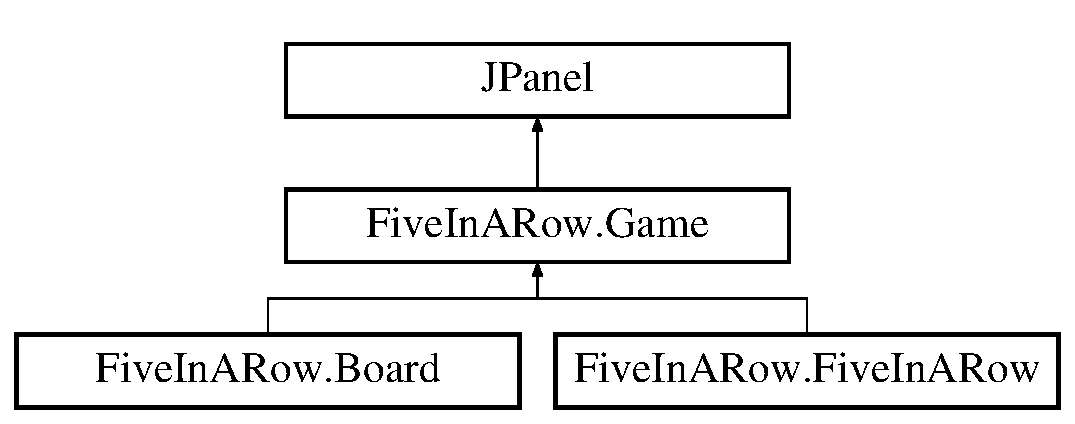
\includegraphics[height=3.000000cm]{class_five_in_a_row_1_1_game}
\end{center}
\end{figure}
\subsection*{Publikus tagfüggvények}
\begin{DoxyCompactItemize}
\item 
void \hyperlink{class_five_in_a_row_1_1_game_a4c602680cf59ce60fa13246477e0e565}{do\+New\+Game} ()
\item 
void \hyperlink{class_five_in_a_row_1_1_game_a25cb45581452401da917ba92fc622a51}{do\+Resign} ()
\item 
void \hyperlink{class_five_in_a_row_1_1_game_ab07617f00f0f27bcc3a6d90f2c6ccd60}{do\+Replay} ()
\item 
void \hyperlink{class_five_in_a_row_1_1_game_a35ea58b4d8584560d43e6847d17d0817}{game\+Over} (String str)
\item 
void \hyperlink{class_five_in_a_row_1_1_game_a34febb68cabf256e603f0ac8b93961f7}{write\+Matrix} (String filename, int\mbox{[}$\,$\mbox{]}\mbox{[}$\,$\mbox{]} matrix)
\end{DoxyCompactItemize}
\subsection*{Statikus publikus tagfüggvények}
\begin{DoxyCompactItemize}
\item 
static void \hyperlink{class_five_in_a_row_1_1_game_a494d022b20310eba3b72f2975ae0f190}{readints} (int\mbox{[}$\,$\mbox{]}\mbox{[}$\,$\mbox{]} matrix, String line, int i)  throws File\+Not\+Found\+Exception 
\end{DoxyCompactItemize}
\subsection*{Publikus attribútumok}
\begin{DoxyCompactItemize}
\item 
\mbox{\Hypertarget{class_five_in_a_row_1_1_game_a1f68c05489c192c40d74d1dc854d3a46}\label{class_five_in_a_row_1_1_game_a1f68c05489c192c40d74d1dc854d3a46}} 
Buffered\+Writer {\bfseries bw}
\item 
\mbox{\Hypertarget{class_five_in_a_row_1_1_game_a4a5ef09201236754a477bfe4ae985f07}\label{class_five_in_a_row_1_1_game_a4a5ef09201236754a477bfe4ae985f07}} 
Buffered\+Reader {\bfseries br}
\end{DoxyCompactItemize}
\subsection*{Statikus publikus attribútumok}
\begin{DoxyCompactItemize}
\item 
\mbox{\Hypertarget{class_five_in_a_row_1_1_game_af8ed6312b46d9f0645db3d3d5f49908f}\label{class_five_in_a_row_1_1_game_af8ed6312b46d9f0645db3d3d5f49908f}} 
static J\+Button {\bfseries new\+Game\+Button}
\item 
\mbox{\Hypertarget{class_five_in_a_row_1_1_game_ac2452fb71ab9d19b9a05e91644d857d6}\label{class_five_in_a_row_1_1_game_ac2452fb71ab9d19b9a05e91644d857d6}} 
static J\+Button {\bfseries resign\+Button}
\item 
\mbox{\Hypertarget{class_five_in_a_row_1_1_game_a3ce1e1d6aaa3233f68346805a672579c}\label{class_five_in_a_row_1_1_game_a3ce1e1d6aaa3233f68346805a672579c}} 
static J\+Button {\bfseries replay\+Button}
\item 
\mbox{\Hypertarget{class_five_in_a_row_1_1_game_a3fda33ad3f7293b311c20780ac1c1c90}\label{class_five_in_a_row_1_1_game_a3fda33ad3f7293b311c20780ac1c1c90}} 
static J\+Label {\bfseries message}
\end{DoxyCompactItemize}


\subsection{Részletes leírás}
Ebben az oszt�lyban a j�t�kkal kapcsolatos met�dusok ker�ltem mint p�ld�ul, �j j�t�k l�trehoz�sa, j�t�k felad�sa, j�t�k visszaj�tsz�sa, j�t�k v�ge �llapot, illetve a visszaj�tsz�sn�l haszn�lt f�jlkezel�s is itt val�sul meg. L�trehozza a t�bl�t a do\+New\+Game met�dusban. \begin{DoxyAuthor}{Szerző}
Roland 
\end{DoxyAuthor}


\subsection{Tagfüggvények dokumentációja}
\mbox{\Hypertarget{class_five_in_a_row_1_1_game_a4c602680cf59ce60fa13246477e0e565}\label{class_five_in_a_row_1_1_game_a4c602680cf59ce60fa13246477e0e565}} 
\index{Five\+In\+A\+Row\+::\+Game@{Five\+In\+A\+Row\+::\+Game}!do\+New\+Game@{do\+New\+Game}}
\index{do\+New\+Game@{do\+New\+Game}!Five\+In\+A\+Row\+::\+Game@{Five\+In\+A\+Row\+::\+Game}}
\subsubsection{\texorpdfstring{do\+New\+Game()}{doNewGame()}}
{\footnotesize\ttfamily void Five\+In\+A\+Row.\+Game.\+do\+New\+Game (\begin{DoxyParamCaption}{ }\end{DoxyParamCaption})}

Elkezd�dik egy �j j�t�k, Ez az action\+Performed() met�dusban h�v�dik meg, amikor a felhaszn�l� az �j j�t�k gombra kattint valamint ind�t�skor a \hyperlink{class_five_in_a_row_1_1_board}{Board} konstruktor�ban. \mbox{\Hypertarget{class_five_in_a_row_1_1_game_ab07617f00f0f27bcc3a6d90f2c6ccd60}\label{class_five_in_a_row_1_1_game_ab07617f00f0f27bcc3a6d90f2c6ccd60}} 
\index{Five\+In\+A\+Row\+::\+Game@{Five\+In\+A\+Row\+::\+Game}!do\+Replay@{do\+Replay}}
\index{do\+Replay@{do\+Replay}!Five\+In\+A\+Row\+::\+Game@{Five\+In\+A\+Row\+::\+Game}}
\subsubsection{\texorpdfstring{do\+Replay()}{doReplay()}}
{\footnotesize\ttfamily void Five\+In\+A\+Row.\+Game.\+do\+Replay (\begin{DoxyParamCaption}{ }\end{DoxyParamCaption})}

A j�t�k visszaj�tsz�s��rt felel�s f�ggv�ny. Ez a met�dus az action\+Performed() met�dusban ker�l megh�v�sra, amikor a felhaszn�l� r�kattint a Replay button-\/ra. Az el�z� j�t�kot/j�t�kokat l�p�sr�l l�p�sre vissza lehet j�tszani a replay gomb lenyom�s�val. Egy gomb nyom�s egy l�p�st j�tszik vissza. \mbox{\Hypertarget{class_five_in_a_row_1_1_game_a25cb45581452401da917ba92fc622a51}\label{class_five_in_a_row_1_1_game_a25cb45581452401da917ba92fc622a51}} 
\index{Five\+In\+A\+Row\+::\+Game@{Five\+In\+A\+Row\+::\+Game}!do\+Resign@{do\+Resign}}
\index{do\+Resign@{do\+Resign}!Five\+In\+A\+Row\+::\+Game@{Five\+In\+A\+Row\+::\+Game}}
\subsubsection{\texorpdfstring{do\+Resign()}{doResign()}}
{\footnotesize\ttfamily void Five\+In\+A\+Row.\+Game.\+do\+Resign (\begin{DoxyParamCaption}{ }\end{DoxyParamCaption})}

A jelenlegi j�t�kos ( current player) feladja a j�t�kot. Ez a met�dus az action\+Performed() met�dusban ker�l megh�v�sra, amikor a felhaszn�l� r�kattint a Resign button-\/ra. A j�t�k v�get �r �s az ellenf�l nyer. \mbox{\Hypertarget{class_five_in_a_row_1_1_game_a35ea58b4d8584560d43e6847d17d0817}\label{class_five_in_a_row_1_1_game_a35ea58b4d8584560d43e6847d17d0817}} 
\index{Five\+In\+A\+Row\+::\+Game@{Five\+In\+A\+Row\+::\+Game}!game\+Over@{game\+Over}}
\index{game\+Over@{game\+Over}!Five\+In\+A\+Row\+::\+Game@{Five\+In\+A\+Row\+::\+Game}}
\subsubsection{\texorpdfstring{game\+Over()}{gameOver()}}
{\footnotesize\ttfamily void Five\+In\+A\+Row.\+Game.\+game\+Over (\begin{DoxyParamCaption}\item[{String}]{str }\end{DoxyParamCaption})}

Ez a met�dus akkor h�v�dik meg amikor a j�t�k v�get �r. Az str param�ter a megjelen�tend� sz�veg. A gombok be �s kikapcsol�dnak, hogy l�tsz�djon a j�t�k m�r nincs folyamatban. 
\begin{DoxyParams}{Paraméterek}
{\em str} & A megjelen�tend� sz�veg. \\
\hline
\end{DoxyParams}
\mbox{\Hypertarget{class_five_in_a_row_1_1_game_a494d022b20310eba3b72f2975ae0f190}\label{class_five_in_a_row_1_1_game_a494d022b20310eba3b72f2975ae0f190}} 
\index{Five\+In\+A\+Row\+::\+Game@{Five\+In\+A\+Row\+::\+Game}!readints@{readints}}
\index{readints@{readints}!Five\+In\+A\+Row\+::\+Game@{Five\+In\+A\+Row\+::\+Game}}
\subsubsection{\texorpdfstring{readints()}{readints()}}
{\footnotesize\ttfamily static void Five\+In\+A\+Row.\+Game.\+readints (\begin{DoxyParamCaption}\item[{int}]{matrix\mbox{[}$\,$\mbox{]}\mbox{[}$\,$\mbox{]},  }\item[{String}]{line,  }\item[{int}]{i }\end{DoxyParamCaption}) throws File\+Not\+Found\+Exception\hspace{0.3cm}{\ttfamily [static]}}

Az el�z� j�t�kok f�jlb�l val� beolvas�sa t�rt�nik a met�dusban. Ez a met�dus a \hyperlink{class_five_in_a_row_1_1_game_ab07617f00f0f27bcc3a6d90f2c6ccd60}{do\+Replay()} met�dusban h�v�dik meg. Amikor vissza szeretn�nk j�tszani egy j�t�kot a Replay gomb megnyom�s�val egyes�vel minden l�p�st beolvas. 
\begin{DoxyParams}{Paraméterek}
{\em matrix} & A matrix param�terhez a t�bl�t kell megadni amibe beolvassuk a l�p�st. \\
\hline
{\em line} & A line param�terben egy beolvasott sort adunk meg amit be�runk a m�trix i. sor�ba. \\
\hline
{\em i} & A line param�terben egy beolvasott sort adunk meg amit be�runk a m�trix i. sor�ba. \\
\hline
\end{DoxyParams}

\begin{DoxyExceptions}{Kivételek}
{\em File\+Not\+Found\+Exception} & Ha nem tal�lja a f�jlt akkor File\+Not\+Fount\+Exceptiont dob. \\
\hline
\end{DoxyExceptions}
\mbox{\Hypertarget{class_five_in_a_row_1_1_game_a34febb68cabf256e603f0ac8b93961f7}\label{class_five_in_a_row_1_1_game_a34febb68cabf256e603f0ac8b93961f7}} 
\index{Five\+In\+A\+Row\+::\+Game@{Five\+In\+A\+Row\+::\+Game}!write\+Matrix@{write\+Matrix}}
\index{write\+Matrix@{write\+Matrix}!Five\+In\+A\+Row\+::\+Game@{Five\+In\+A\+Row\+::\+Game}}
\subsubsection{\texorpdfstring{write\+Matrix()}{writeMatrix()}}
{\footnotesize\ttfamily void Five\+In\+A\+Row.\+Game.\+write\+Matrix (\begin{DoxyParamCaption}\item[{String}]{filename,  }\item[{int}]{matrix\mbox{[}$\,$\mbox{]}\mbox{[}$\,$\mbox{]} }\end{DoxyParamCaption})}

A t�bla vagyis a m�trix f�jlba val� �r�sa itt t�rt�nik, az a visszaj�tsz�s miatt sz�ks�ges. A met�dus a do\+Click\+Square() met�dusban h�v�dik meg. Teh�t minden l�p�s ut�n ki�rja egy f�jlba a jelenlegi �ll�st, amit majd k�s�bb vissza tudunk olvasni, a visszaj�tsz�shoz.


\begin{DoxyParams}{Paraméterek}
{\em filename} & A filename param�ter a f�jl nev�t jelenti amibe �rni fogunk. \\
\hline
{\em matrix} & A matrix param�ter pedig a t�bl�t amit lement�nk a f�jlba. \\
\hline
\end{DoxyParams}


Ez a dokumentáció az osztályról a következő fájl alapján készült\+:\begin{DoxyCompactItemize}
\item 
Game.\+java\end{DoxyCompactItemize}

%--- End generated contents ---

% Index
\backmatter
\newpage
\phantomsection
\clearemptydoublepage
\addcontentsline{toc}{chapter}{Tárgymutató}
\printindex

\end{document}
